\customchapter[January 10, 2023]{Lecture 3: Deterministic Finite Acceptors}

\section{Language from grammer}

\begin{example}
    Consider the grammer $ \bbG = ( \{s\} , \{a, b\} , \bbS, \bbP ) ; \quad \bbP_1 \bbS \rightarrow a \bbS b / \lm $ then language generated by this grammer is $$\bbL(G_1) = \{ a^mb^m : m \geq 0 \} $$
\end{example}

\begin{example}
    Consider the grammer $ \bbG = ( \{s, \bbA \} , \{a, b\} , \bbS, \bbP ) ; \quad \bbP_2 \bbS \rightarrow a \bbS b / \lm, \bbA \rightarrow a \bbA b / \lm $ then language generated by this grammer is $$\bbL(G_2) = \{ a^mb^m : m \geq 0 \} $$
\end{example}

\begin{definition}{}
    Two grammers are equivalent iff $L(G_1) = L(G_2)$
\end{definition}

\section{Deterministic Finite Acceptors (DFA)}

\begin{definition}{}
    A DFA is defined by $\bbM = ( \bbQ, \Sigma, \bbD, \bbQ_0, \bbF )$ where \begin{itemize}
        \item $\bbQ$ is a finite set of states
        \item $\Sigma$ is a finite set of input symbols
        \item $\bbD : \bbQ \times \bbE \rightarrow \bbQ$ is a transition function
        \item $\bbQ_0 \in \bbQ$ is the start state
        \item $\bbF \subseteq \bbQ$ is the set of final states
    \end{itemize}
\end{definition}

\begin{example}
    Consider the DFA $ \bbM = ( \{q_0, q_1, q_2\} , \{a, b\} , \bbD, q_0, \{q_1\} ). \\  \bbD(q_0, a) = q_1, \bbD(q_0, b) = q_0, \bbD(q_1, a) = q_2, \bbD(q_1, b) = q_0, \bbD(q_2, a) = q_2, \bbD(q_2, b) = q_2 $
\end{example}

\section{Graphical Representation of DFA}

\begin{definition}{}
    A DFA is represented by a directed graph $G = (V, E)$ where \begin{itemize}
        \item $V = \bbQ$
        \item $E = \{ (q, \bbD(q, \bbE), \bbE) : q \in \bbQ, \bbE \in \bbE \}$
        \item an open $\rightarrow$ indicates the start state
        \item $\bigcirc$ indicates the final state 
    \end{itemize}
\end{definition}

\begin{example}
    Consider the DFA $ \bbM = ( \{q_0, q_1, q_2\} , \{a, b\} , \bbD, q_0, \{q_1\} ). \\  \bbD(q_0, a) = q_1, \bbD(q_0, b) = q_0, \bbD(q_1, a) = q_2, \bbD(q_1, b) = q_0, \bbD(q_2, a) = q_2, \bbD(q_2, b) = q_2 $   
\end{example}

\begin{figure}[!h]
    \centering
    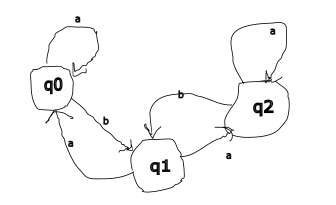
\includegraphics[width=0.5\textwidth]{figures/graphical_1.png}
    \caption{DFA}
\end{figure}

